%%==================================================
%% chapter03.tex for TJU Master Thesis
%% Encoding: UTF-8
%%==================================================

\chapter{软管组件加强层理论发展综述}


\section{引~言}


%目前对金属编织加强软管的研究,多见于汽车工业中的中刹车管[2]、转向传动管[3]、空调管[4] 等。

软管组件作为一种上世纪中叶,就开始广泛使用的重要工业构件,
事实上,对其的研究一直以实验、实用为主,没有形成一套通用完整的体系。图\ref{fig:hose-system-theories}描述了软管组件的理论路线和分支。

\begin{figure}[!htbp]
\centering
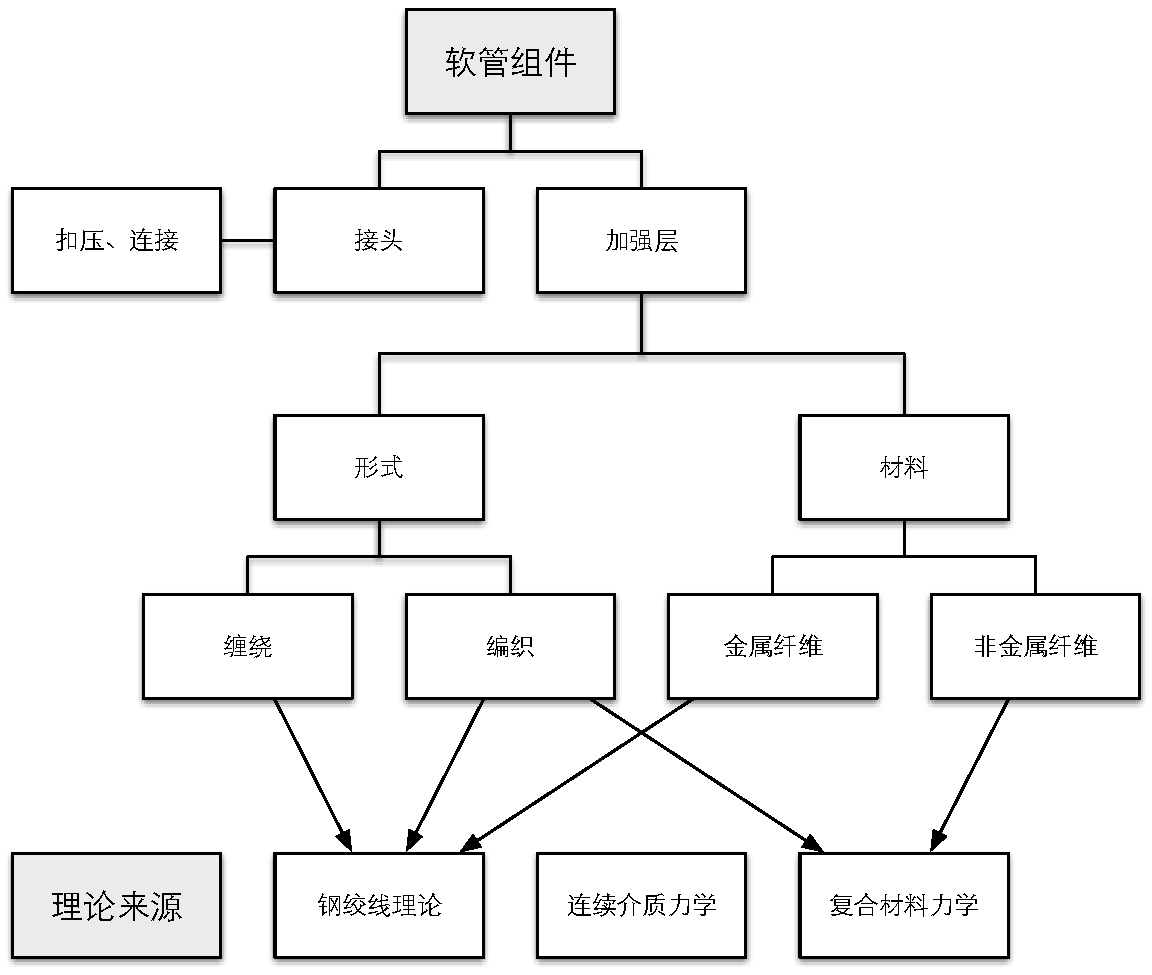
\includegraphics[width=0.7\linewidth]{figure/chap3/理论体系}
	\fcaption{软管组件理论体系}{Hose Assembly Theory Branches}
	\label{fig:hose-system-theories}
\end{figure}

软管组件的理论与研究首先分为两个对象:
\begin{inparaenum}[1).]
	\item 接头
	\item 加强层。
\end{inparaenum}
本文的研究主要针对加强层,这里不对软管组件的连接技术进行阐述。而加强层包含了缠绕、编织两种形式,又包括了金属纤维、非金属纤维两种材料,理论界并没有明确和统一的认识,而是基于各自不同的理论之上。

加强层的理论研究成果,主要是建立在三个理论体系之上的,包括了
\begin{inparaenum}[1).]
	\item 钢绞线理论
	\item 复合材料力学
	\item 连续介质力学
\end{inparaenum}



\section{理论分支概述}
钢绞线理论,来源于悬索、电缆等结构。钢绞线理论应用于加强层的力学分析,有两个主要的分支\cite{Evans2002}:
\begin{inparaenum}[1).]
	\item 加强层含量较低,橡胶管起主要作用的软管,由\citeauthor{Kuipers1989}等人[6,7]提出并完善,适用于帘线加强的软管;
	\item 加强层主要承力的软管,主要研究的是高密度钢丝缠绕加强层。
\end{inparaenum}
这套理论体系成熟与上世纪90年代初,适用于金属纤维的缠绕层,编织层一般作为缠绕层的一种扭转为0的特殊情况。前文提到的第一代、第二代软管组件一般是以这套理论指导设计的。

随着第三代非金属加强软管组件的大量使用,近20年来,对编织加强结构的研究主要集中在复合材料编织。复合材料纤维编织的与金属纤维编织的传力机制差别非常明显[8],研究方法的也有所区别:钢绞线理论一般以钢丝为载体;复合材料一般采用特征元法作为力学分析的对象。复合材料理论中有大量简化编织结构的理论,许多学者选择其中适合软管加强层的理论开展了工作



也有学者尝试用连续介质力学的基本理论推导编织层的本构,\citeauthor{Horgan2005}\cite{Horgan2005} 提出了纤维加强材料的应变能密度函数,
国内学者计算了编织结构强度与突加荷载的情况\cite{2009b}。

但是,主流的研究办法还是结合实验,提出能够反映加强层力学行为的有限元模型。\citeauthor{Wijaya2012}\cite{Wijaya2012}对包含软管各层材料及编织层的试件进行了压缩实验,认为金属编织层的应力应变关系是线性的,在软管整体动态特性的研究中取得了较好的效果。\citeauthor{Cho2005}\cite{Cho2005}研究了编织层在扣压安装接头中的力学行为,结合压缩实验提出了弹塑性的本构模型,\citeauthor{Rattensperger2003}\cite{Rattensperger2003}同样针对压缩的过程,编织层厚度方向引入一组等效非线性弹簧,表征金属纤维间相互作用。



\section{基于钢绞线理论的研究}


%stepI hruska 
\citeauthor{hruska1951calculation}\cite{hruska1951calculation,hruska1952radial,hruska1953tangential}分析了钢绞线结构中一层钢丝的轴向、切向以及径向的应力。钢绞线中一层钢丝实际上就是一层螺旋缠绕结构,也被用于早期设计软管组件缠绕层的参考依据。而其理论并没有考虑结构半径的变化,也没有考虑钢绞线排布的角度$ \alpha_i $的变化。也就是说,该理论不能考虑编织层受内压后,结构的几何变化。该理论仅考虑了钢绞线的拉伸刚度,扭转和弯曲的刚度皆为0。钢绞线体系轴向拉力$ T_\alpha $与单根钢丝轴线拉力$ T_i $的关系为:
\begin{equation}
T_\alpha = T_i \cos{\alpha_i}
\end{equation}

1951年,\citeauthor{hruska1951calculation}也给出了单位长度径向力$ F_{RU} $与钢绞线拉力$ T $、钢丝曲率半径$ \rho $关系的表达式,如式\ref{eq:Hruska}所示。该理论提出时仅作为实验得到的经验公式,后在\citeyear{machida1973}由\citeauthor{machida1973}给出证明。

\begin{equation}\label{eq:Hruska}
{F_{RU}} = \frac{T}{\rho }
\end{equation}
其中,钢丝的曲率半径可以由螺旋缠绕的结构参数表征
\begin{equation}
\rho  = \frac{R}{{{{\sin }^2}{\alpha _i}}}
\end{equation}
$ R_i $为钢绞线总体半径。


1977年,\citeauthor{Entwistle1977}\cite{Entwistle1977}针对编织加强软管,提出了一套更为准确的理论假设。这套理论相对之前的理论,可以考虑缠绕层受内压荷载后,结构的几何变化。\citeauthor{Entwistle1977}对加强层几何变化的假设如图\ref{fig:assumption-deformed-geometry}所示,该理论不允许软管发生扭转,这是考虑到在该理论体系下编织层的扭转必须为0。

加强层变形前后的半径为$ R_i $、$ R_i' $,缠绕角为$ \alpha_i$ 、 $\alpha_i' $,钢丝应变为$ \varepsilon_i $,之间的关系可以通过图\ref{fig:assumption-deformed-geometry}中的几何关系表示

\begin{equation}
\frac{{{R_i}'}}{{{R_i}}} = \left( {1 + {\varepsilon _i}} \right)\frac{{\sin {\alpha _i}'}}{{\sin {\alpha _i}}}
\end{equation}

\begin{figure}[!htbp]
	\centering
		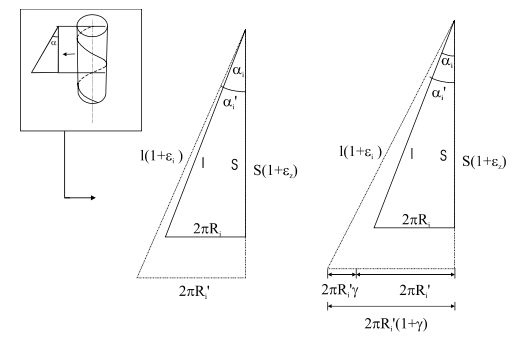
\includegraphics[width=0.7\linewidth]{figure/chap3/review/a}
	\fcaption{加强层几何变化假设}{Assumption for the deformed reinforcement geometry}
	\label{fig:assumption-deformed-geometry}
\end{figure}

1979年,\citeauthor{Knapp1979}\cite{Knapp1979}针对内芯可压缩的钢绞线结构进行了研究,采用了和\citeauthor{machida1973}(\citeyear{machida1973})相似的手段,引入了扭转因子$ \gamma_i $(图\ref{fig:assumption-deformed-geometry}),其表达式为:
\begin{equation}
{R_i}' = {R_i}\frac{{\left( {1 + {\varepsilon _i}} \right)\sin {\alpha _i}'}}{{\left( {1 + {\gamma _i}} \right)\sin {\alpha _i}}}
\end{equation}

这个分支下的研究,实际上还是围绕着加强结构中的钢丝本身,没有一个平均化的概念,所得的结果也是加强层中的某根钢丝与结构整体位移、扭转的关系。而且该系列理论主要研究的是缠绕加强,编织总是被简化为特殊的缠绕。编织远比缠绕来得复杂,很多复编织层特有的复杂关系、结构都被过度简化,也不能很好得融入该理论体系。

\section{基于复合复合材料理论的研究}














\section{数值解法的发展}




\section{拉伸实验与软管}


很早就有学者用拉伸实验开始研究纤维加强层。\citeauthor{brunnschweiler19545}\cite{brunnschweiler19545}用拉伸试验机对不同编织角的的编织层进行了测试。他们发现使得编织结构失效的拉伸量,至少是编织层所用纤维失效拉伸量的$ 150\% $以上。单位面积内的股数与编织层失效拉伸量正相关,同样也与初始编织角相关。


\cite{Hajrasouliha1}



\citeauthor{Leung2013}\cite{Leung2013}


采用了双镜头显微摄像仪(stereomicroscope)以及数字图像修正技术(digital image correlation,DIC)研究了拉伸实验,扫描了复合材料编织层表面的三维模型,记录了拉伸时表面的型位移场、编织角,研究了复合材料加强硬管拉伸时的编织角变化和基体裂纹的生长。

\citeauthor{Harte20001259}\cite{Harte20001259,Harte2000259}研究了符合材料编织层拉伸时的力学行为和颈缩现象。他们也利用层合板理论预测了编织层的弹性模量。他们同时也提出:编织结构能非常有效的吸收能量,在拉伸过程中,编织层发生较大的拉伸应变时,纤维上的拉伸应变是恒定值。



\section{本文研究思路}